\documentclass[12pt, oneside]{report}\usepackage[]{graphicx}\usepackage[]{color}
% maxwidth is the original width if it is less than linewidth
% otherwise use linewidth (to make sure the graphics do not exceed the margin)
\makeatletter
\def\maxwidth{ %
  \ifdim\Gin@nat@width>\linewidth
    \linewidth
  \else
    \Gin@nat@width
  \fi
}
\makeatother

\usepackage{Sweavel}


\usepackage[margin=0.85in]{geometry}
\linespread{1}
\usepackage{xcolor}
\usepackage[colorlinks=false, linkbordercolor=white, citebordercolor=white, 
    filebordercolor=white, urlbordercolor=white]{hyperref}
    
\usepackage{graphicx}
\usepackage[utf8]{inputenc}
\usepackage[english]{babel}
\usepackage[T1]{fontenc}

\usepackage{fancyhdr}
\pagestyle{fancy}
\renewcommand{\headrulewidth}{0.4pt}
\fancyhead{}
\fancyhead[L]{Course Name -- assignment 1} %%% change to your course name and change the number accordingly
\fancyhead[R]{First Name Surname} %%% change to your first name and surname
\fancyfoot{}
\fancyfoot[C]{\thepage}

\usepackage{titlesec}
\titlespacing{\chapter}{0pt}{*4}{*2.5}

\titleformat{\chapter}{\normalfont\huge\bf}{\thechapter}{20pt}{\huge\bf}


% Setting up of environment
\usepackage{listings}
\definecolor{dgray}{gray}{0.35} % colour of comments
\definecolor{lgray}{gray}{0.95} % background colour of R-code
\definecolor{llgray}{gray}{0.98} % background colour of R-outputs

\lstdefinestyle{Rstyle}{ % settings of R-code style
language=R, % setting language R
basicstyle=\ttfamily\small, % font and size of R-code
backgroundcolor=\color{lgray}, % background colour of R-code
commentstyle=\ttfamily\small\itshape\color{dgray}, % colour of R comments
showstringspaces=false, % forbidding the highlighting of spaces
numbers=left, % numbering on the left
numberstyle=\ttfamily\small, % font and size of numbering
stepnumber=1, % numbering with step 1
firstnumber=last, % cumulative numbering of rows in consecutive Chunks
breaklines=T} % automatic line breaks of code at the end of a line

\lstdefinestyle{Routstyle}{ %  settings of R-output style
language=R, % setting language R
basicstyle=\ttfamily\small, % font and size of R-output
backgroundcolor=\color{llgray}, % background colour of R-code
showstringspaces=false, % forbidding the highlighting of spaces
numbers=right, % numbering on the right
numberstyle=\ttfamily\small, % font and size of numbering
firstnumber=last, % cumulative numbering of rows in consecutive Chunks
breaklines=T} % automatic line breaks of code at the end of a line

\begin{document}



\begin{titlepage}
    \begin{center}
        \vspace*{1cm}
        
        \Huge
          \textbf{Course Name} %%% change to your course name
        
        \vspace{0.5cm}
        \LARGE
        Assignment 1 %%% change the number accordingly
        
        \vspace{1.5cm}
        
        \textbf{First Name Surname} %%% change to your first name and surname
   		  \vspace{1.5cm}
        
        \textbf{UCO} %%% change to your UCO
       
        \vfill
        
        Field of Study XY %%% change to your field of study
        
        \vspace{0.8cm}
          \Large
        Faculty of Informatics\\
        Masaryk University\\
        \vspace{0.5cm}
       \today
        
    \end{center}
\end{titlepage}

\addtocontents{toc}{~\hfill\textbf{Page}\par}

\section*{Exercise 1}
\noindent Text. Commentary on the approach to solving the exercise, theoretical derivation if the assignment asks for it.

Text. Paragraphs are separated by an empty line.

\subsection*{Implementation in R}

\begin{Schunk}
\begin{Sinput}
## this is so called chunk, where you write R-code, including loading data and libraries
library(xtable)

baschar <- function(x){
  ## function for computing number of observations, mean and standard deviation
  # input: x ... vector of observations
  # output: vector containing number of observation, mean and standard deviation
  v1 <- c(length(x), mean(x), sd(x))
  return(v1)
}

obs <- rnorm(100,0,5)
characteristics <- baschar(obs)
char.mat <- matrix(characteristics, nrow=1, dimnames = list('name of variable', c('n', '$\\overline{x}$', '$s$')))
\end{Sinput}
\end{Schunk}

\bigskip

\subsection*{Results and interpretation}
\noindent Text. Results in table or graphic form. Commentaries and interpretation of the results.

Interpretation. Text. Commentary relating to tables and figures. 

% latex table generated in R 3.6.3 by xtable 1.8-4 package
% Fri Apr 10 23:33:40 2020
\begin{table}[ht]
\centering
\begin{tabular}{|l|rrr|}
  \hline
 & n & $\overline{x}$ & $s$ \\ 
  \hline
name of variable & 100 & 0.37 & 5.31 \\ 
   \hline
\end{tabular}
\caption{Characteristics of (name of variable)} 
\end{table}


\begin{Schunk}
\begin{Sinput}
hist(obs, main='', xlab='name of variable', ylab='frequency')
\end{Sinput}
\begin{figure}[h]

{\centering 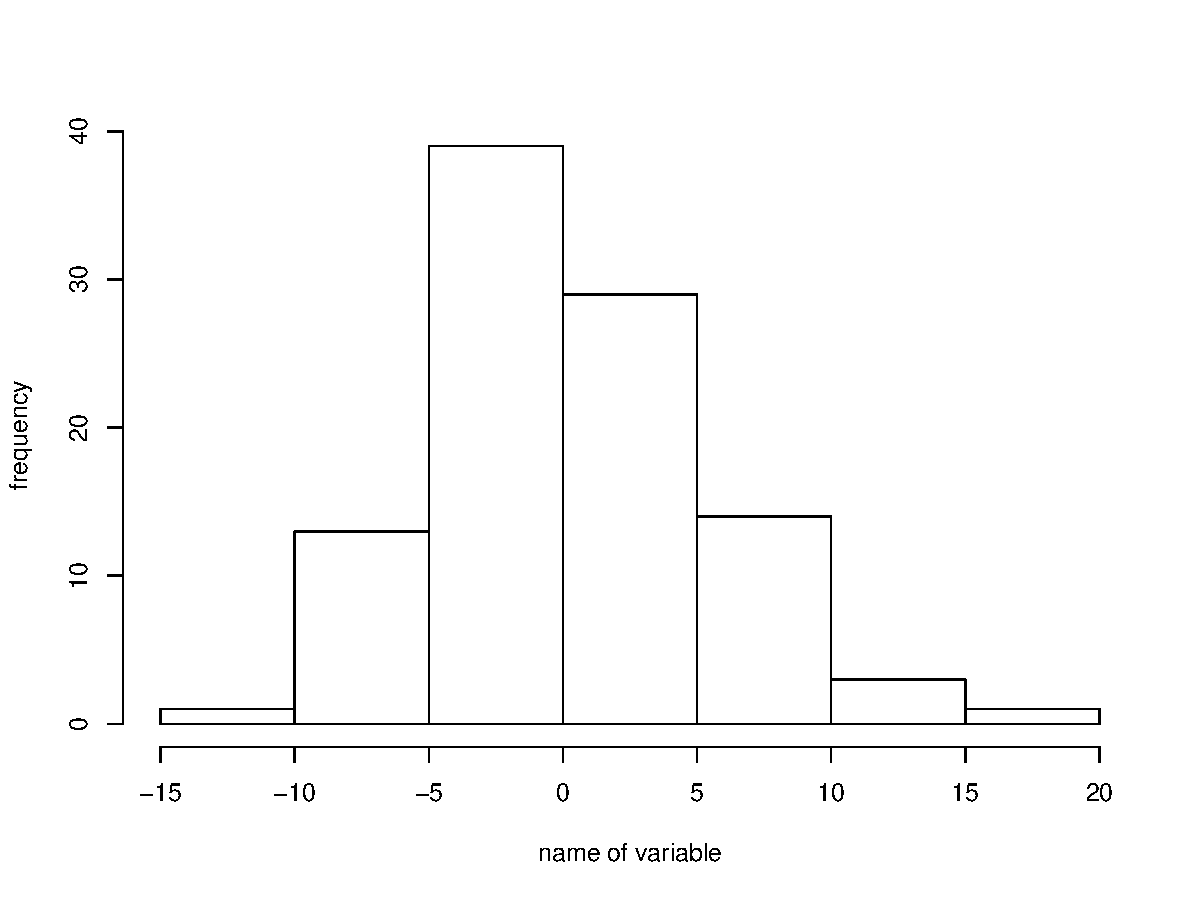
\includegraphics[width=.6\textheight,height=.45\textheight]{figure/unnamed-chunk-3-1} 

}

\caption[Histogram of (name of variable)]{Histogram of (name of variable)}\label{fig:unnamed-chunk-3}
\end{figure}
\end{Schunk}


\newpage

\section*{Exercise 2}
\noindent Don't forget to check, whether you included all required outputs in each exercise.

\end{document}
